\section{Numerical states that distinguish time intervals}\label{sec:numerical}

The scheduler uses the same coordinates in many disjoint intervals.
Each interval must have a recognizable set of coordinates at zero. It
must also be possible to interpolate between successive samples using
convex inequalities. We construct finite sets of nonnegative vectors
that meet both requirements.

Call the intervals \emph{sites}, and number them from \(1\) to \(L\).
A \emph{layer} is a sample position in their linear order. Each site
has a blank layer at either end and any positive number of intervening
layers, called \emph{micro layers}. The last blank of one site and the
first blank of the next are distinct.

\begin{theorem}[Numerical layer theorem]\label{thm:coarse}
Fix integers \(r\ge100\) and \(C\ge1000r^2\). There are arbitrarily
large powers of two \(q\) with the following property. Set \(L_0=q^C\)
and \(L=L_0^m\) for any sufficiently large integer \(m\). Let \(b\)
be the least power of two at least \(L^{1/(r+1)}\), and let
\(\mathcal A\) be a nonempty set of at most \(b\) positions.
There are a finite index set \(\mathcal I\) and maps
\(\mathrm h_a:\{1,\ldots,L\}\to\mathbb F_b\) for \(a\in\mathcal A\)
such that
\[
 |\mathcal I|\le L^{8/C},\qquad
 \big|\{a:\mathrm h_a(s)=\mathrm h_a(s')\}\big|\le r
 \quad(s\ne s').
\]
Index coordinates by labels \(\ell=(i,a,t)\) in
\(\mathcal I\times\mathcal A\times\mathbb F_b\). The \emph{bundle}
with index \(i\) at site \(s\) is
\(H_i(s)=\{(i,a,\mathrm h_a(s)):a\in\mathcal A\}\).
For any numbers of micro layers, each layer \(j\) admits a finite
nonempty set \(\mathcal S_j\) of vectors in the unit cube on these
labels, called \emph{states}, with the following properties.
\begin{enumerate}
\item Given states \(u\in\mathcal S_{j-1}\) and
\(v\in\mathcal S_{j+1}\) on either side of any layer \(j\), some
\(y\in\mathcal S_j\) satisfies
\begin{equation}\label{eq:layermerge}
                y_\ell\le\tfrac14\max\{u_\ell,v_\ell\}
                \quad\text{at every label }\ell .
\end{equation}
\item Every state at a micro layer of site \(s\) vanishes on one
entire \(H_i(s)\). On each \(H_{i'}(s')\) with \(s'\ne s\) it has
at most \(r\) zero coordinates.
\item The number of states per layer is bounded independently of all
site lengths. If there are \(n_L\) layers, every positive state entry
has the form \(4^{-k}\) for an integer \(0\le k\le c_0 n_L\);
\(c_0\) may depend on \(r,C,q,m,\mathcal A\).
\end{enumerate}
\end{theorem}

The coordinates will record how often a path changes direction while
avoiding a specified label. To see what paths are needed, imagine
building a state at each layer and repeatedly adjoining the states
required by Equation~\eqref{eq:layermerge}. A binary expression
records the history of each such operation.

\subsection{Binary terms and a one-scale marking lemma}

A \emph{term} is a finite rooted binary expression with a layer
assigned to each node. Each layer has a leaf term. At an interior
layer a new term can be formed by merging any term in the preceding
layer (its west parent) with any term in the following layer (its
east parent). These rules generate all terms. A path follows parent
links and includes both its endpoints. A \emph{turn} is a change of
direction between consecutive links. The west and east \emph{spines}
of a term follow the respective parent at each step until a leaf is
reached.

We will also use terms on a contiguous block of layers. To \emph{clip}
a term to a block containing its root, replace each node first reaching
either boundary layer of the block by the leaf in that layer. The paths
of the clipped term follow the same parent links as in the original
term up to their endpoints. On such a path, clipping the original
subterm at any visited node gives precisely its subterm in the clipped
expression.

The next lemma provides a random mark on a fixed number \(L_0\) of
sites. Every micro term receives the mark with a specified minimum
probability. From any blank term there is a path to a leaf that
encounters the mark in at most one other site. Sections~\ref{sec:probability}--\ref{sec:finite}
give the construction and proof.

\begin{lemma}[Primary Lemma]\label{lem:primary}
For each integer \(C\ge50\) there are arbitrarily large powers of two
\(q\) with the following property. For \(L_0=q^C\) sites there is a
finite probability space \(\Omega\) independent of the numbers of
micro layers. For any choice of those numbers, each term \(v\) can
be assigned a set \(P(v)\subseteq\Omega\) such that
\begin{enumerate}
\item \(P(v)=\varnothing\) on every blank layer and
\(\Pr(P(v))\ge q^{-5}\) on every micro layer.
\item For every blank term in site \(s\) and every \(\omega\in\Omega\),
there is a path from that term to a leaf on which all terms \(v\)
with \(\omega\in P(v)\) lie in a single site different from \(s\).
There may be no such terms. The number of turns is bounded in terms
of \(C,q\) alone.
\end{enumerate}
\end{lemma}

\subsection{Distinguishing sites at successive scales}

Choose \(q\) from Lemma~\ref{lem:primary} large enough that
\(2\log_2 L_0\le q\). Partition the \(L=L_0^m\) sites into blocks
of \(L_0\) consecutive sites. Group \(L_0\) consecutive blocks into
a larger block, repeating until the entire sequence forms one block.
Number the levels from \(1\) to \(m\), starting with the finest blocks.
At each level above the first, a site is a whole block from the previous
level. Regard its first and last layers as blanks and all intervening
layers as micro layers. Apply the Primary Lemma to the \(L_0\) sites
in every block, clipping terms to that block. A term \(v\) on a finest
micro layer is micro at every level and thus has \(m\) sets of marks of
measure at least \(q^{-5}\).

There is a fixed list \(\mathcal T\subseteq\Omega^m\) of size at most
\(q^{7m}\) that meets every product of \(m\) subsets of \(\Omega\)
whose individual measures are at least \(q^{-5}\). Indeed, \(q^{7m}\)
independent tuples sampled from the product measure miss any such
product with probability at most \(\exp(-q^{2m})\). There are at most
\(2^{m|\Omega|}\) products. Since \(\Omega\) was fixed before \(m\),
their total failure probability is less than one for all sufficiently
large \(m\).

Within each block write its site numbers \(0,\ldots,L_0-1\) in binary,
using \(\log_2 L_0\) bits per number. An index \(i\) consists of a
tuple in \(\mathcal T\) and, for each level, a bit position and a bit
value. Thus the set \(\mathcal I\) of possible indices satisfies
\begin{equation}\label{eq:tensor-index-size}
        |\mathcal I|\le q^{7m}(2\log_2 L_0)^m
        \le q^{8m}=L^{8/C}.
\end{equation}
We assign one index to each finest micro term and none to the finest
blank terms. We say that a term \emph{emits} its assigned index.
At every level the tuple entry of an emitted index must be a mark of
the clipped term, and the recorded bit must match the address of its
site. We now choose the bits so that these two necessary conditions
exclude repeated emissions along a suitable path.

\begin{lemma}\label{lem:emission-escape}
The assignment can be made so that from every term emitting \(i\)
there is a path to a leaf on which all emissions of \(i\) occur in
its starting finest site. The number of turns on this path is bounded
independently of the term and the site lengths.
\end{lemma}
\begin{proof}
At a finest micro term \(v\), choose a tuple from \(\mathcal T\)
belonging to all \(m\) sets of marks. Follow one spine in the starting
site as far as a leaf or the first blank. If a blank is reached, apply
Lemma~\ref{lem:primary} there in the level-one block, with the first
entry of the tuple. On the resulting path all occurrences of that mark
lie in a single different site. Choose a bit where the addresses of the
two sites differ, and record the starting site's value. If the mark
never occurs, any position with its correct value suffices. On this
segment a term therefore either lacks the required mark or fails the
bit test. Figure~\ref{fig:layer-bits} illustrates the choice.

Lift the path from the clipped term to the original term. If the endpoint
is a genuine leaf, stop. Otherwise it is an exterior blank of the
level-one block, and therefore a blank of the starting site at level two.
Repeat with the next tuple entry. The preceding clipping observation
ensures that the marks tested on a lifted segment agree with the ones
used to decide whether its terms may emit the index. At the last level
an exterior blank is a global endpoint and necessarily a genuine leaf.
For any unused levels record an arbitrary correct bit. The initial
spine stays within the starting finest site, and each subsequent
segment excludes the index. There are at most \(m\) such segments,
each with the bounded number of turns from the Primary Lemma, and at
most \(m\) joining turns. The choices at \(v\) depend only on addresses
and marks, so they can be made at every micro term independently.
\end{proof}

\begin{figure}[htbp]
\centering
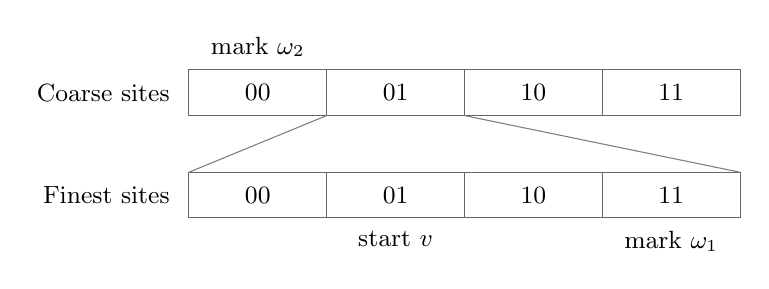
\begin{tikzpicture}[x=1cm,y=1cm,font=\small]
  \foreach \j/\bits in {0/00,1/01,2/10,3/11}{
    \draw[black!60] ({1.75*\j},1.3) rectangle ({1.75*\j+1.75},1.88);
    \draw[black!60] ({1.75*\j},0) rectangle ({1.75*\j+1.75},.58);
    \node at ({1.75*\j+.875},1.59) {\(\bits\)};
    \node at ({1.75*\j+.875},.29) {\(\bits\)};
  }
  \node[anchor=east] at (-.12,1.59) {Coarse sites};
  \node[anchor=east] at (-.12,.29) {Finest sites};
  \draw[black!50] (1.75,1.3)--(0,.58);
  \draw[black!50] (3.5,1.3)--(7,.58);
  \node[anchor=south] at (.875,1.92) {mark \(\omega_2\)};
  \node[anchor=north] at (2.625,-.05) {start \(v\)};
  \node[anchor=north] at (6.125,-.05) {mark \(\omega_1\)};
\end{tikzpicture}
\caption{Choosing an address bit at each of two levels. Within the
starting coarse site \(01\), the finest site of \(v\) is \(01\) and
the first mark occurs only in \(11\) along the first escape segment.
Recording the first bit of \(01\) excludes \(11\). On the next
segment the second mark occurs only in coarse site \(00\). The second
bit of the starting coarse site \(01\) excludes its entire block.}
\label{fig:layer-bits}
\end{figure}

\subsection{Numerical slack from paths}

Assign distinct polynomials of degree at most \(r\) over \(\mathbb F_b\)
to the \(L\) sites, and evaluate each polynomial at distinct field elements
indexed by \(\mathcal A\) to obtain the tags \(\mathrm h_a(s)\). This is
the polynomial evaluation construction of Reed and Solomon~\cite{reedsolomon}.
There are \(b^{r+1}\ge L\) polynomials, and two distinct polynomials agree
at at most \(r\) positions. Whenever a term at site \(s\) emits \(i\),
regard it as emitting each label in \(H_i(s)\).

\begin{proof}[Proof of Theorem~\ref{thm:coarse}]
For a term \(v\) and label \(\ell\), consider all paths from \(v\) to a
leaf that avoid emission of \(\ell\) at every term, including \(v\).
A path of zero steps has cost zero. For a nonempty path \(\pi\), write
\(\partial_\pi\) for the global boundary layer in the direction of its
first step and define
\begin{equation}\label{eq:turn-cost}
 c(\pi)=1+\operatorname{dist}(v,\partial_\pi)
                   +3n_L\,\operatorname{turns}(\pi),
\end{equation}
where distance counts layer steps. Prepending a step increases the cost
by at least one. In the original direction the distance increases by one.
In the opposite direction a new turn contributes \(3n_L\), exceeding any
loss in the distance term. Prepending to an empty path also increases
the cost.

Choose \(c_0\) so that the cutoff \(c_0 n_L\) bounds the cost of a
spine followed by a path from Lemma~\ref{lem:emission-escape}, including
the turn at the join. The lemma bounds the number of turns independently
of \(n_L\). If the minimum cost of an avoiding path is \(k\le c_0 n_L\),
put \(y_\ell(v)=4^{-k}\). If there is no such path below or at the cutoff,
put \(y_\ell(v)=0\). Let \(\mathcal S_j\) consist of the vectors \(y(v)\)
of all terms in layer \(j\). Each layer has a leaf, so its set is
nonempty. At a fixed layer the first direction has two choices and the
number of turns below the cutoff is bounded in terms of \(c_0\). Thus
Equation~\eqref{eq:turn-cost} allows only boundedly many exponents for
each coordinate. The number of labels is independent of the site
lengths, giving the asserted uniform state count.

Given states at the two neighbors of a layer, merge terms carrying those states.
A positive entry \(4^{-k}\) of the merge has an avoiding path of cost
\(k\). Removing its first step gives one parent an avoiding path of cost
at most \(k-1\), so that parent's entry is at least \(4\cdot4^{-k}\).
Thus the merged vector satisfies Equation~\eqref{eq:layermerge}. At a
micro term its own emission cannot be avoided, so the state vanishes on
the entire emitted bundle.

Finally fix an index \(i\) and a micro term at site \(s\). If a spine
from the term reaches a leaf without an emission of \(i\), that one
path avoids every label with first component \(i\) within the cutoff.
Otherwise denote the sites of the first emissions on the west and east
spines by \(s_-\) and \(s_+\). At the first emission on each spine,
continue along the path of Lemma~\ref{lem:emission-escape}. The new
paths stay below the cutoff and can encounter labels of index \(i\)
only in \(H_i(s_-)\) and \(H_i(s_+)\), respectively. Every zero of
index \(i\) therefore lies in \(H_i(s_-)\cap H_i(s_+)\). If either
site equals \(s\), its intersection with a foreign bundle contains at
most \(r\) labels by polynomial evaluation. Otherwise \(s_-\) is
strictly west of \(s\) and \(s_+\) strictly east, so even
\(H_i(s_-)\cap H_i(s_+)\) has at most \(r\) labels in total.
\end{proof}
